% This is a template for your written document.
%
% To compile using latexmk on the command line, run the following: 
% latexmk -pdf main.tex

\documentclass[12pt]{article}
\usepackage{setspace}
\singlespace
\usepackage[left=1in,right=1in,top=1in,bottom=1in]{geometry}
\usepackage{graphicx}

\title{\textbf{Reflective AI Feedback for Personal Productivity}}
\author{Saidamir Osimov}

\begin{document}

\maketitle

\section{Introduction}
Productivity systems are everywhere.They have become deeply embedded in the daily life of millions of people, whether they work
 in the office, schools, or a project. They help maintain consistency and track tasks and goals. By reviewing someone's schedule 
 and task list in their productivity app, you can learn a great deal about them, such as how busy they are throughout the week, how 
 productive they are each day, and how many meetings and tasks they have. Task managers, digital planners, goal tracking dashboards, and
  habit-building apps: users now have multiple tools to organize their life and structure their time. All these platforms are great
   at dividing the work into actionable small steps, setting deadlines and monitoring completion rates across different horizons.
     While they are great at tracking and supporting execution, they rarely foster insight. Users can rigorously record what they do, 
     but they receive little to no support in understanding how they work.


At the rate of tasks and pressure of commitments, individuals face cognitive overload. When tasks are completed, postponed, or 
rescheduled, it is often done so without any coherent decision-making behind them. Productivity tools generate data about the
 person more than ever before, but they provide minimal awareness about behavioral patterns, motivational cycles, or attention
  shifts. Tracking an activity is not the same as understanding it. Without systems for reflection, productivity tools are more like 
  sophisticated record keepers rather than instruments for self-improvement.

\subsection{ The Need for Reflective Feedback }
Reflection plays an important role in cognitive growth and sustained performance. Research in the field of cognitive science 
consistently shows that individuals improve not just by completing tasks, but by investigating how and why they approach them. 
In particular, a 2025 study, “Effect of feedback-integrated reflection on deep learning of medical students” \cite{Maqsood2025}, 
found that combining structured reflection with feedback caused significantly higher learning gains (approximately 69\% compared 
to 29\%). The study also highlights how reflective feedback reinforces metacognitive activity, enabling learners to monitor thinking
 and adjust behaviors effectively. When individuals look back and analyze patterns in their performance and attention, they develop 
 awareness that supports more goal-aligned action.

Although, reflective practice is widely supported by research, most productivity platforms remain focused on task completion and 
execution rather than metacognitive development(awareness and understanding of your own thought process). Although users can record 
activities and track results, they are rarely encouraged to analyze their patterns or get personalized feedback. The absence of
 smart reflection systems shows a major disconnect between what cognitive science knows and what productivity tools actually offer.

Recent progress in artificial intelligence(AI), particularly large language models(LLMs) allow productivity systems to go beyond task 
management, toward cognitive support. Unlike traditional software, artificial intelligence can analyze large volumes of data and
 detect patterns across time and interpret contextual details in user generated logs. This allows the system to make sense of 
 information rather than just collecting it. Large language models are capable of identifying recurring themes in work behavior, 
 demonstrating inconsistencies between stated goals and actual actions, and generating reflection feedback in natural language.
  Artificial intelligence can help users to interpret their own patterns of focus, procrastination, prioritization, and energy
   allocation. In this sense artificial intelligence functions as a mechanism for cognitive augmentation. By letting intelligent 
   systems handle pattern recognition and reflection, users can develop self-awareness without having to do all the mental heavy
    lifting themselves.


\subsection{	Introducing Newton}
Newton is a productivity system designed to have artificial intelligence driven reflective feedback directly into the everyday 
workflow management. Built on top of the Supermind Design concept introduced by MIT\cite{10.1145/3643562.3672611}, the platform
 encourages creative thinking and intentional execution rather than passive task tracking. The core functionality of Newton lies
 in its analysis of user activity through structured change logs. 
As users edit tasks, mark them complete and update goals, these changes are then captured and interpreted by an integrated 
artificial intelligence component. The system analyzes the logs to detect recurring patterns and inconsistencies. Based on
 this analysis, Newton generates personalized reflective insights that help users to zoom out of the daily routine and evaluate
  how their actions are aligned with their long-term goals. Rather than simply reporting what has been completed, the system 
  highlights how your work develops over time and where you might need to adjust.
This project explores how integrating AI-generated reflective feedback into productivity systems can enhance user awareness, 
improve workflow efficiency, and support more intentional decision-making.

\section{Background}
The Supermind Design method is humans and computers working together to generate better solutions to solve problems. Rather than 
replacing human thinking, these systems combine human creativity and judgement with computational power of the machines. Also, the
 Supermind Design is an approach to problem solving that combines big picture thinking with creative and intentional actions. Rather 
 than focusing on isolated tasks, this method encourages individuals to view components to treat problems as parts of a larger, 
 connected whole rather than standalone issues to fix.  A key part of this approach is looking at things from different angles, and 
 considering both the small details and the bigger picture before making any decisions. By stepping back before diving into the 
 details users can better spot root problems, and hidden issues that might be missed with a narrow focus. Supermind Design also
  promotes iterative reflection rather than strictly following a plan. Reframing plays a key role in this method, encouraging users 
  to question assumptions and find alternative solution paths. This framework blends human intuition with structured reasoning.

\subsection{Supermind Design in Newton}
Newton applies the Supermind Design principles by combining human decision making with artificial intelligence generated insights. 
Instead of operating only as a task manager the system is designed to support the collaboration between the user and the artificial
 intelligence systems, that give reflective feedback and analyze the behavioral patterns.
By analyzing the logs, the artificial intelligence component is able to help users see the patterns over time in their day-to-day 
work. This is the reflection of Supermind Design: combining humans with computational analysis to get better insights on productivity
 and workflow.

Artificial intelligence does not replace humans; it enhances them. The invention of the calculator did not replace the need for
 mathematicians, or math ability; it sped it up. An LLM does not replace thinking; it improves and supports reasoning. Newton is
  not doing the work for the user, it is helping them see the patterns in their own behavior and empowering them to look at their
   workflow from another perspective. That is augmentation. Artificial intelligence expands cognitive capacity. 

A tool waits for the instructions, Newton is more like a partner that: 1) Observes 2) Suggests 3) Reflects. Traditional productivity
 apps are passive, Newton on the other hand is reflective. That is the difference. If I ask Siri a question, then it will give me 
 an answer. I use Newton, it analyzes my behavior through the progress logs and tells me: “You tend to overcommit midweek” or “You
  abandon long-term tasks after 5 days”.(Conclusion)





\section{Related Works}
Researchers have intensely studied how artificial intelligence systems can support task management and everyday work activities. 
Work by D. Trippas 
and colleagues \cite{10.1145/3295750.3298934} categorizes common workplace tasks to help design intelligent assistants that better 
understand the goals of the users and their activities. The study demonstrates that there are common patterns in work activities and
 tasks. Most commonly they involve multiple step tasks, goals and contextual factors.
Other research \cite{KHAOKAEW2022102905} on future digital assistants in the workplace suggests that users want tools that are not
 just reactive tools but also adaptive supporters of complex work processes.
Traditional digital assistants respond to commands and perform tasks. However, these studies indicate that the workers increasingly
 expect the assistants to understand context and support planning and decision making. On the same topic, Newton analyzes user task
  history and change logs to generate reflective feedbacks. Instead of simply following the commands, it aims to help users 
  understand the patterns in their workflow and support them in more informed decision making.

Recent research frames artificial intelligence as a tool for augmented human cognition, rather than replacing human decision making.
 This means that, artificial intelligence is used to help humans think better and support them in decision making.
  For example, Supermind Ideator developed by Thomas W. Malone and collaborators \cite{10.1145/3643562.3672611} showcases how 
structured human and artificial intelligence collaboration can improve creative problem solving. By offering support such as 
rephrasing problems, prompting new ideas, and guiding collaboration, the system helped users come up with significantly more
 creative ideas than when working alone or using regular AI tools. Similarly, research on the ExtendAI framework by Leon Reicherts 
 and colleagues \cite{10.1145/3706598.3713295} shows that 

AI systems are more effective when they extend and support users' reasoning processes rather than simply providing recommendations.
 Their findings suggest that AI tools that integrate with users' own decision-making strategies lead to better engagement and 
 slightly improved outcomes. Research by Xiaotong Xu \cite{10.1145/3706598.3713649} also shows that adding AI to creative 
 workflows can help users generate more ideas and explore problems more deeply.

Together, these studies point to a bigger shift in how artificial intelligence systems are being designed. The goal is always
 to support human thinking, not replace it. Newton takes this same approach by integrating AI into everyday productivity workflows,
  using data and task history to help users reflect on and improve their work habits.




%\begin{figure}[b] puts the image to the (closest) bottom of page
%\begin{figure}[t] puts the image to the (closest) top of page
%\begin{figure}[h] allows the image to float, putting it roughly wherever it was placed in the text.

\section{Methodology}
Newton is developed as a reflective productivity system that tracks not only what users accomplish, but also how they accomplish 
it over time. Instead of being a typical task manager that prioritizes execution and completion, Newton is more focused on pattern 
recognition and behavioral analysis. This is done to shift the usual task tracking toward deeper self-awareness. The system analyzes
 user activity, aiming to help individuals understand their habits, inconsistencies between planned goals and actual behavior, and
  decision-making. 
  Artificial intelligence in Newton is used as a form of cognitive augmentation, helping users understand the information about 
  their own workflow that would otherwise be difficult to track manually over time. By showcasing behavioral patterns and providing 
  reflective feedback to users, Newton encourages them to step back and evaluate their work and make more intentional decisions on 
  how to spend energy and time on tasks more efficiently.

A key feature of Newton's approach lies in its ability to record any change made in the platform regarding tasks and user activity 
over time. The system continuously logs any changes made in the platform in the Progress panel. These changes include events such as 
task creation, task completion, deletion, rescheduling, and edits along with their timestamps. Instead of treating each task as a 
single isolated action, these logs create a continuous record of how a user behaves and interacts with their own workflow, reflecting
 the real behavior. For instance, if a user frequently reschedules a task, it may be an indicator of overcommitment. Similarly, 
 repeated edits may suggest uncertainty or shifting priorities. By collecting this information about the user, Newton is able to go 
 beyond simple tracking and begin identifying behavioral patterns. This provides a foundation for generating reflective insights for
  users to better understand how they perform over time.


To turn raw activity logs into meaningful insights, Newton uses a large language model to interpret the behavior. The system
 provides the model with the change logs and a prompt that frames the task as reflective rather than directive. The prompt 
 encourages the model to analyze the patterns in the behavior of the user, along with inconsistencies and trends. Depending on 
 the implementation, this model may be deployed locally or accessed through an external API, with each option presenting trade-offs
  in terms of privacy, cost, and performance. Instead of just summarizing the data, the goal is to help the user be more aware of 
  their workflow and behavioral trends, such as overcommitment, delays in task completion, and shifts in priorities.


The output is shown to the user in the form of structured feedback, organized as bullet points for readability. The insights are 
personalized and are directly related to the user's recent activity on Newton, making them more relevant. For instance, the system 
might highlight uneven workload distribution across the week, or inconsistencies between the stated goals and the accomplished goals. 
The system intentionally avoids giving instructions, instead providing reflective feedback that encourages the user to interpret and 
respond based on their own judgement. This reinforces the role of Newton as a cognitive supporter rather than augmenter. By 
presenting the feedback in a clear format, we help the user to quickly grasp the patterns in their behavior, avoiding the need for 
manual analysis.

\section{Implementation}
Newton is built as a web-application that combines the UI with the AI analysis tool. The system collects and stores user 
interactions locally using browser storage. Actions such as creating, editing, completing, or rescheduling tasks are recorded and 
used as the primary data source. When enough activity is collected, it is passed to a language model, which identifies patterns and 
generates reflective feedback. This creates a straightforward pipeline: raw interaction data is logged, analyzed, and returned to 
the user as meaningful insights.


The interface design of Newton is inspired by 
the Timestripe productivity application, infinite horizontal timeline feature in particular. Users can scroll infinitely to the left 
to view past days and to the right to plan future tasks, with each day represented as a column. Tasks are organized within these day
 columns, allowing users to visually structure their workflow over time. The application is composed of several key components,
  including a Sidebar for navigation, a Horizon panel \ref{fig:horizon}  for task planning, a Progress panel \ref{fig:progress} for viewing activity logs, and an AI 
  Insights panel \ref{fig:reflection} for reflective feedback. The Horizon panel allows users to create and manage tasks across different dates, while
   the Progress panel records and organizes all changes made within the system. The AI Insights panel then presents the generated
    reflections based on this data. Together, these components create a continuous loop where user actions are recorded, analyzed,
     and reflected back in a way that supports awareness and adjustment.

From the implementation perspective, the system is structured using a component-based architecture in React. The main application 
initializes the interface and manages state, including storing tasks as date-keyed objects and maintaining change logs. Components 
such as DayColumn and TaskItem handle task-level interactions, while the TaskModal provides a more detailed editing interface. Data 
persistence is handled through local storage, allowing user activity to be retained across sessions without requiring a backend. For
 the AI component, the current implementation uses a locally deployed DeepSeek 7B model to generate insights. While this approach 
 offers advantages in terms of privacy and control, it introduces latency, with response times of several minutes. Future iterations
  may explore external API-based models, such as ChatGPT, which could significantly reduce response time at the cost of reduced data 
  locality and potential privacy considerations.

  Newton extends the Horizon panel by introducing multiple time scales, including day, week, month, and year views. Each of these 
  sub-panels operates on the same structural principle, where tasks are grouped into time-based columns, but they serve different 
  planning purposes. This allows users to shift between short-term execution and long-term planning without changing the underlying
   interaction model. A key feature within each column is the ability to generate AI-driven insights directly from that specific
    time frame. By clicking an insight trigger within a column, the system collects completed tasks within that period and sends 
    them to the language model for analysis. This enables localized reflection, where users can evaluate productivity at different 
    temporal resolutions, such as understanding how a single day compares to a full week or month.

In addition to a default system prompt that frames the AI as a productivity coach, Newton allows users to customize the prompt used 
for generating insights \ref{fig:insight}. This design choice introduces flexibility and user control into the reflection process. While the default
 prompt focuses on general productivity patterns, users can modify it to emphasize specific goals, such as time management, focus, 
 or consistency. At the same time, the system provides an option to reset to the original prompt, ensuring that users can always 
 return to a stable baseline. This feature reflects an important design principle: reflection should not be imposed in a single 
 rigid format, but instead adapted to individual preferences and needs. By allowing users to shape how the AI interprets their data,
  Newton moves closer to a personalized cognitive support system

  Newton also includes a dedicated AI Insights panel \ref{fig:reflection} that functions as a conversational interface. Unlike the column-based insights,
   which are tied to a specific time window, this panel has access to the full activity history of the user. It allows users to ask 
   open-ended questions about their productivity, such as comparing performance across weeks or identifying trends over longer
    periods. The system constructs a summarized activity log from recorded events and provides it to the language model along with 
    the ongoing conversation. This enables more dynamic and context-aware interactions, where users can explore their behavior
    through iterative questioning. The chat-based interface transforms reflection from a passive experience into an interactive 
    process, allowing users to actively engage with their data rather than simply receiving static feedback.


Newton also introduce more flexible task management features, such as drag-and-drop reordering and cross-column movement. Users can 
rearrange tasks within a column to reflect changing priorities, or move tasks across different days and time frames. Additionally,
 incomplete tasks are automatically carried over to the next day, ensuring continuity in planning. While these features primarily
  improve usability, they also provide additional behavioral signals for analysis. For example, frequent reordering may indicate 
  shifting priorities, while repeated carryover of tasks may highlight overcommitment or unrealistic planning. By capturing these
   interactions, the system gains a more nuanced understanding of user behavior beyond simple task completion.


\subsection{The model}
The current implementation uses locally deployed language models, including DeepSeek 7B and the Gemma model family. These models are
 particularly effective for reasoning tasks, as they are designed to handle structured input and generate coherent, step-by-step
  interpretations. In the context of Newton, this makes them well-suited for identifying behavioral patterns within activity logs,
   such as recurring delays, uneven workload distribution, or inconsistencies between goals and actions. Their ability to process 
   sequences of events and generate natural language explanations allows the system to translate raw data into meaningful insights. 
   Running the models locally also provides advantages in terms of privacy and control, as user data does not need to be sent to 
   external servers. However, this comes at the cost of increased latency, with response times ranging from one to several minutes.


\section{Results}
The current version of Newton demonstrates that it is possible to transform raw productivity data into meaningful reflective 
feedback using AI. In practical use, the system is able to identify patterns such as frequent task rescheduling, uneven workload
 distribution across days, and gaps between planned and completed tasks. These insights are presented in a concise and structured 
 format, making them easy for users to interpret. Early informal testing suggests that users are able to recognize aspects of their
  behavior that were previously unnoticed, particularly in relation to overcommitment and shifting priorities.

The introduction of multi-scale insights further improves the usefulness of the system. By allowing users to generate feedback at 
the level of a day, week, or month, Newton supports both short-term and long-term reflection. Users can observe how daily habits 
accumulate into broader patterns over time. Additionally, the conversational AI interface enables more flexible exploration of
 productivity data. Instead of relying solely on predefined insights, users can ask targeted questions and receive context-aware 
 responses based on their activity history. Together, these features demonstrate the potential of combining structured data logging
  with AI-driven interpretation.


\section{Analysis and Discussion}



\section{Conclusion}



\begin{figure}[h]
  \centering
  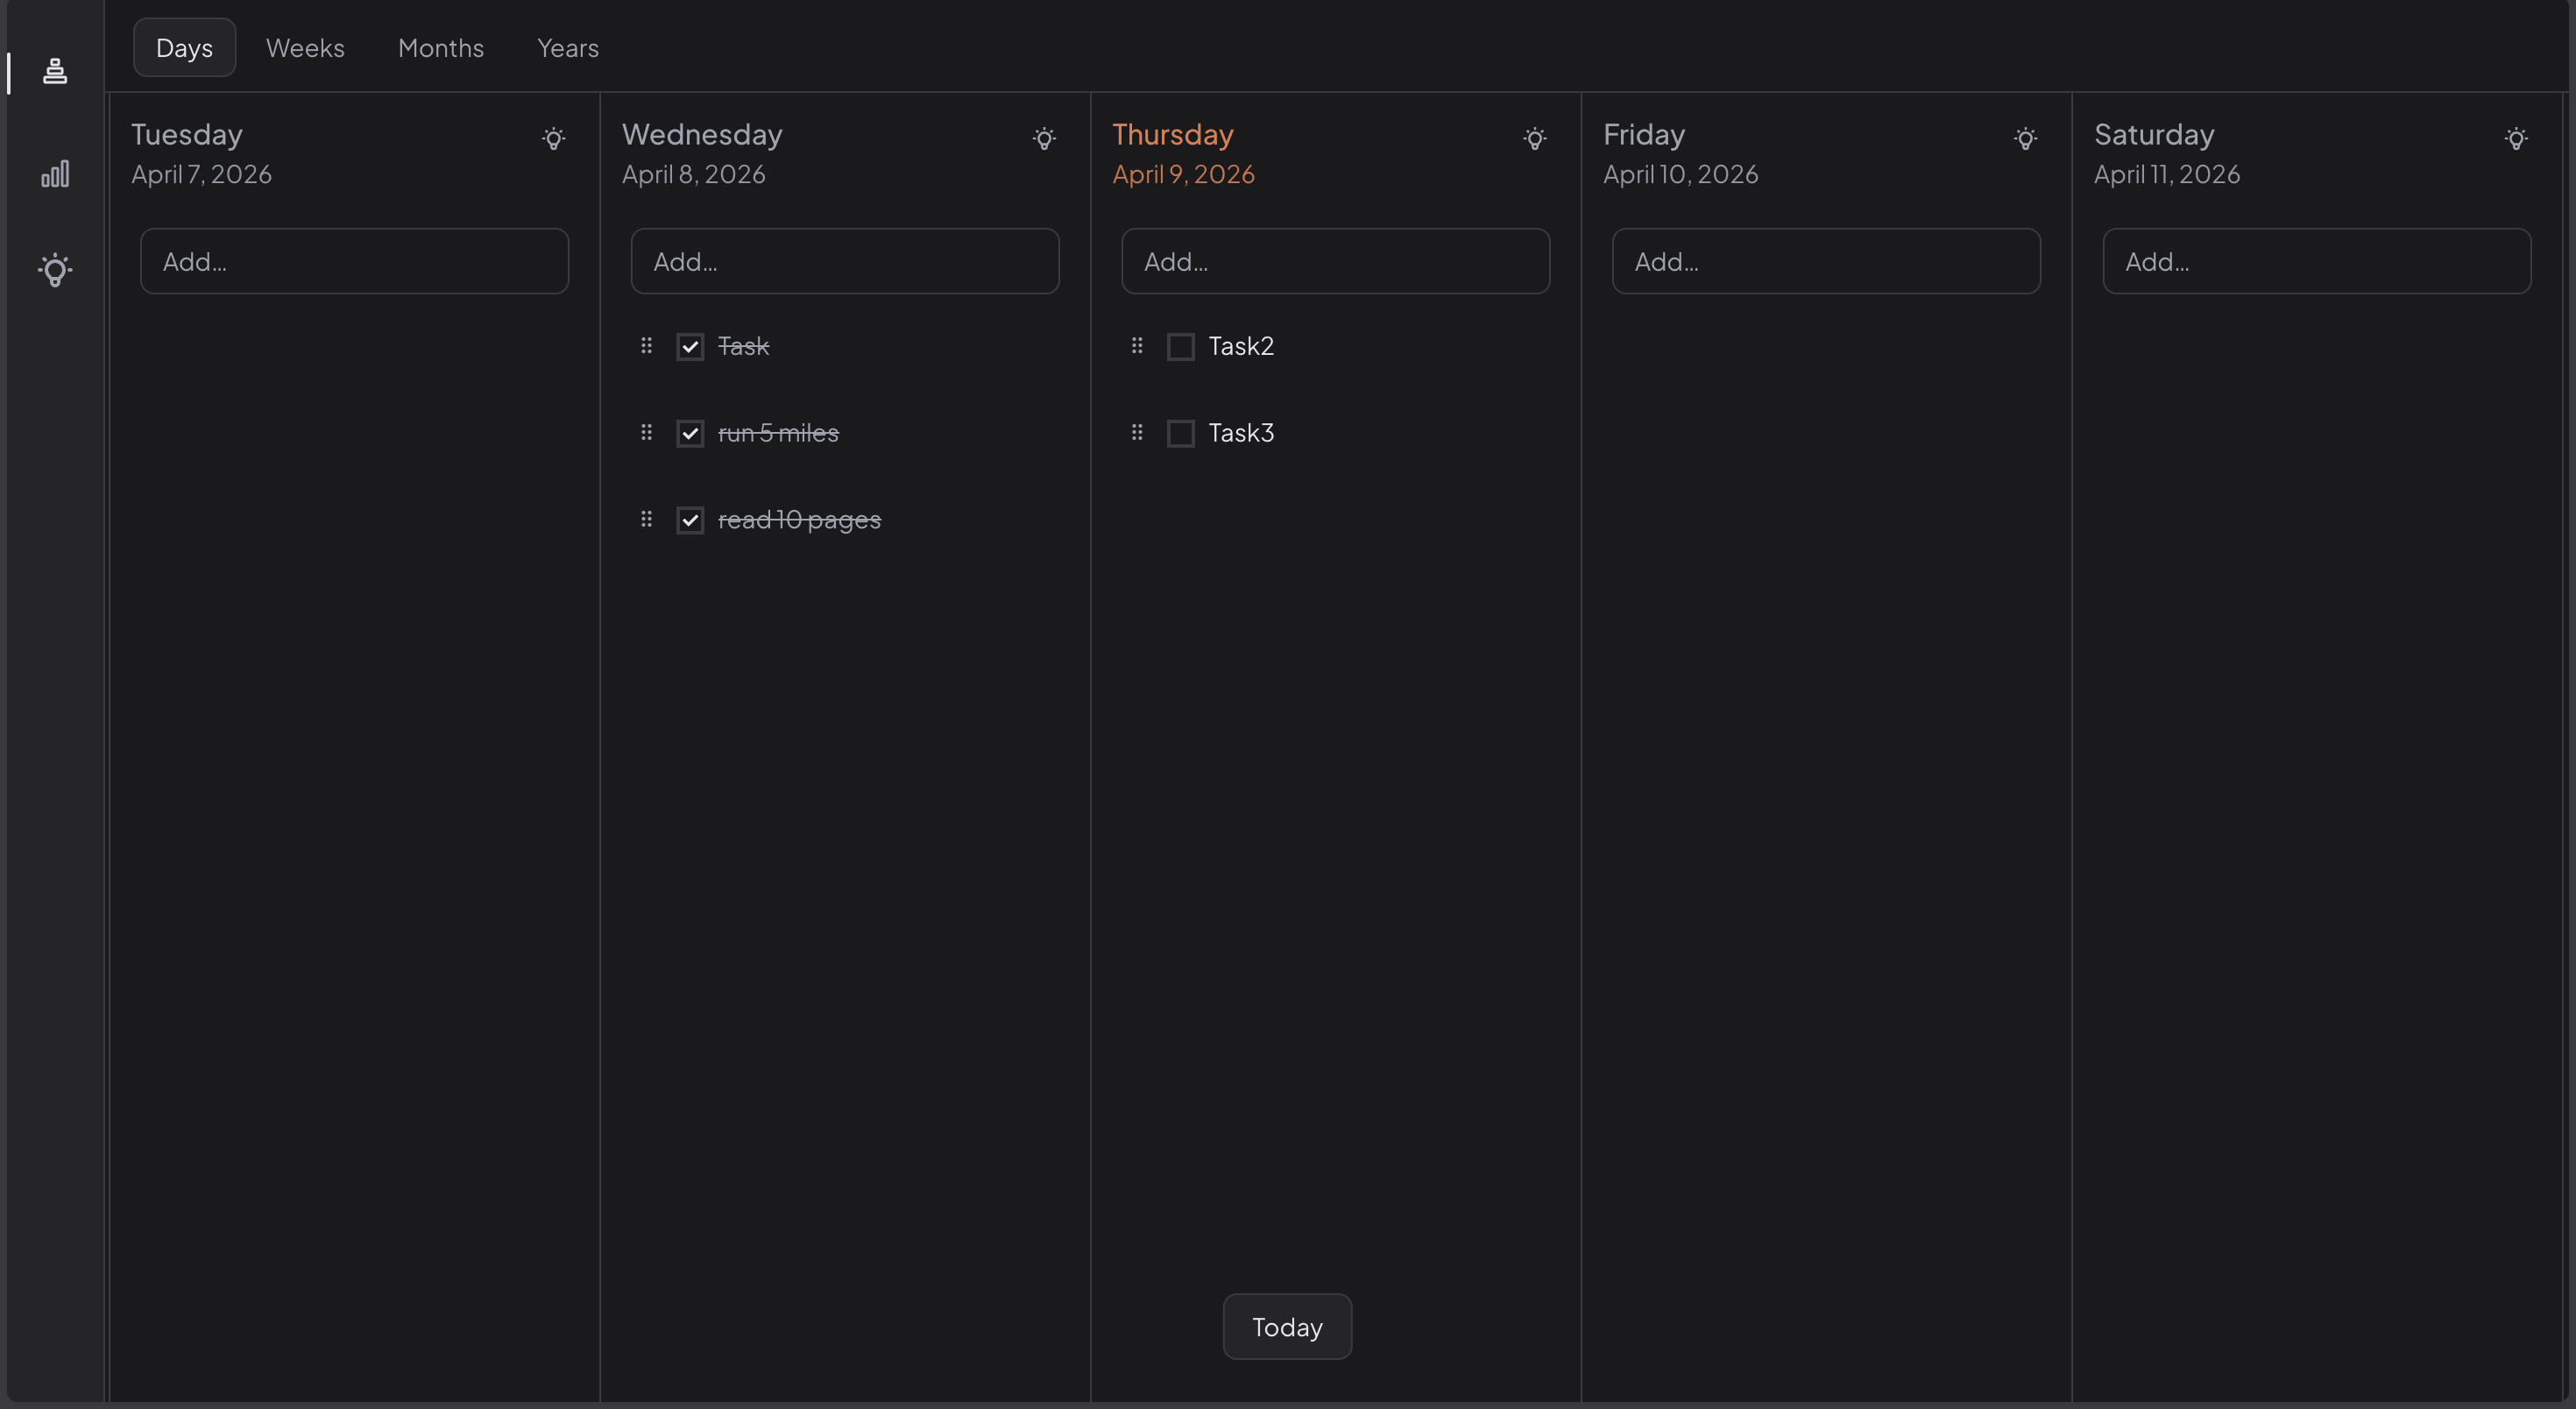
\includegraphics[width=0.8\linewidth]{Horizon.png}
  \caption{Horizon Panel}
  \label{fig:horizon}
\end{figure}

\begin{figure}[h]
  \centering
  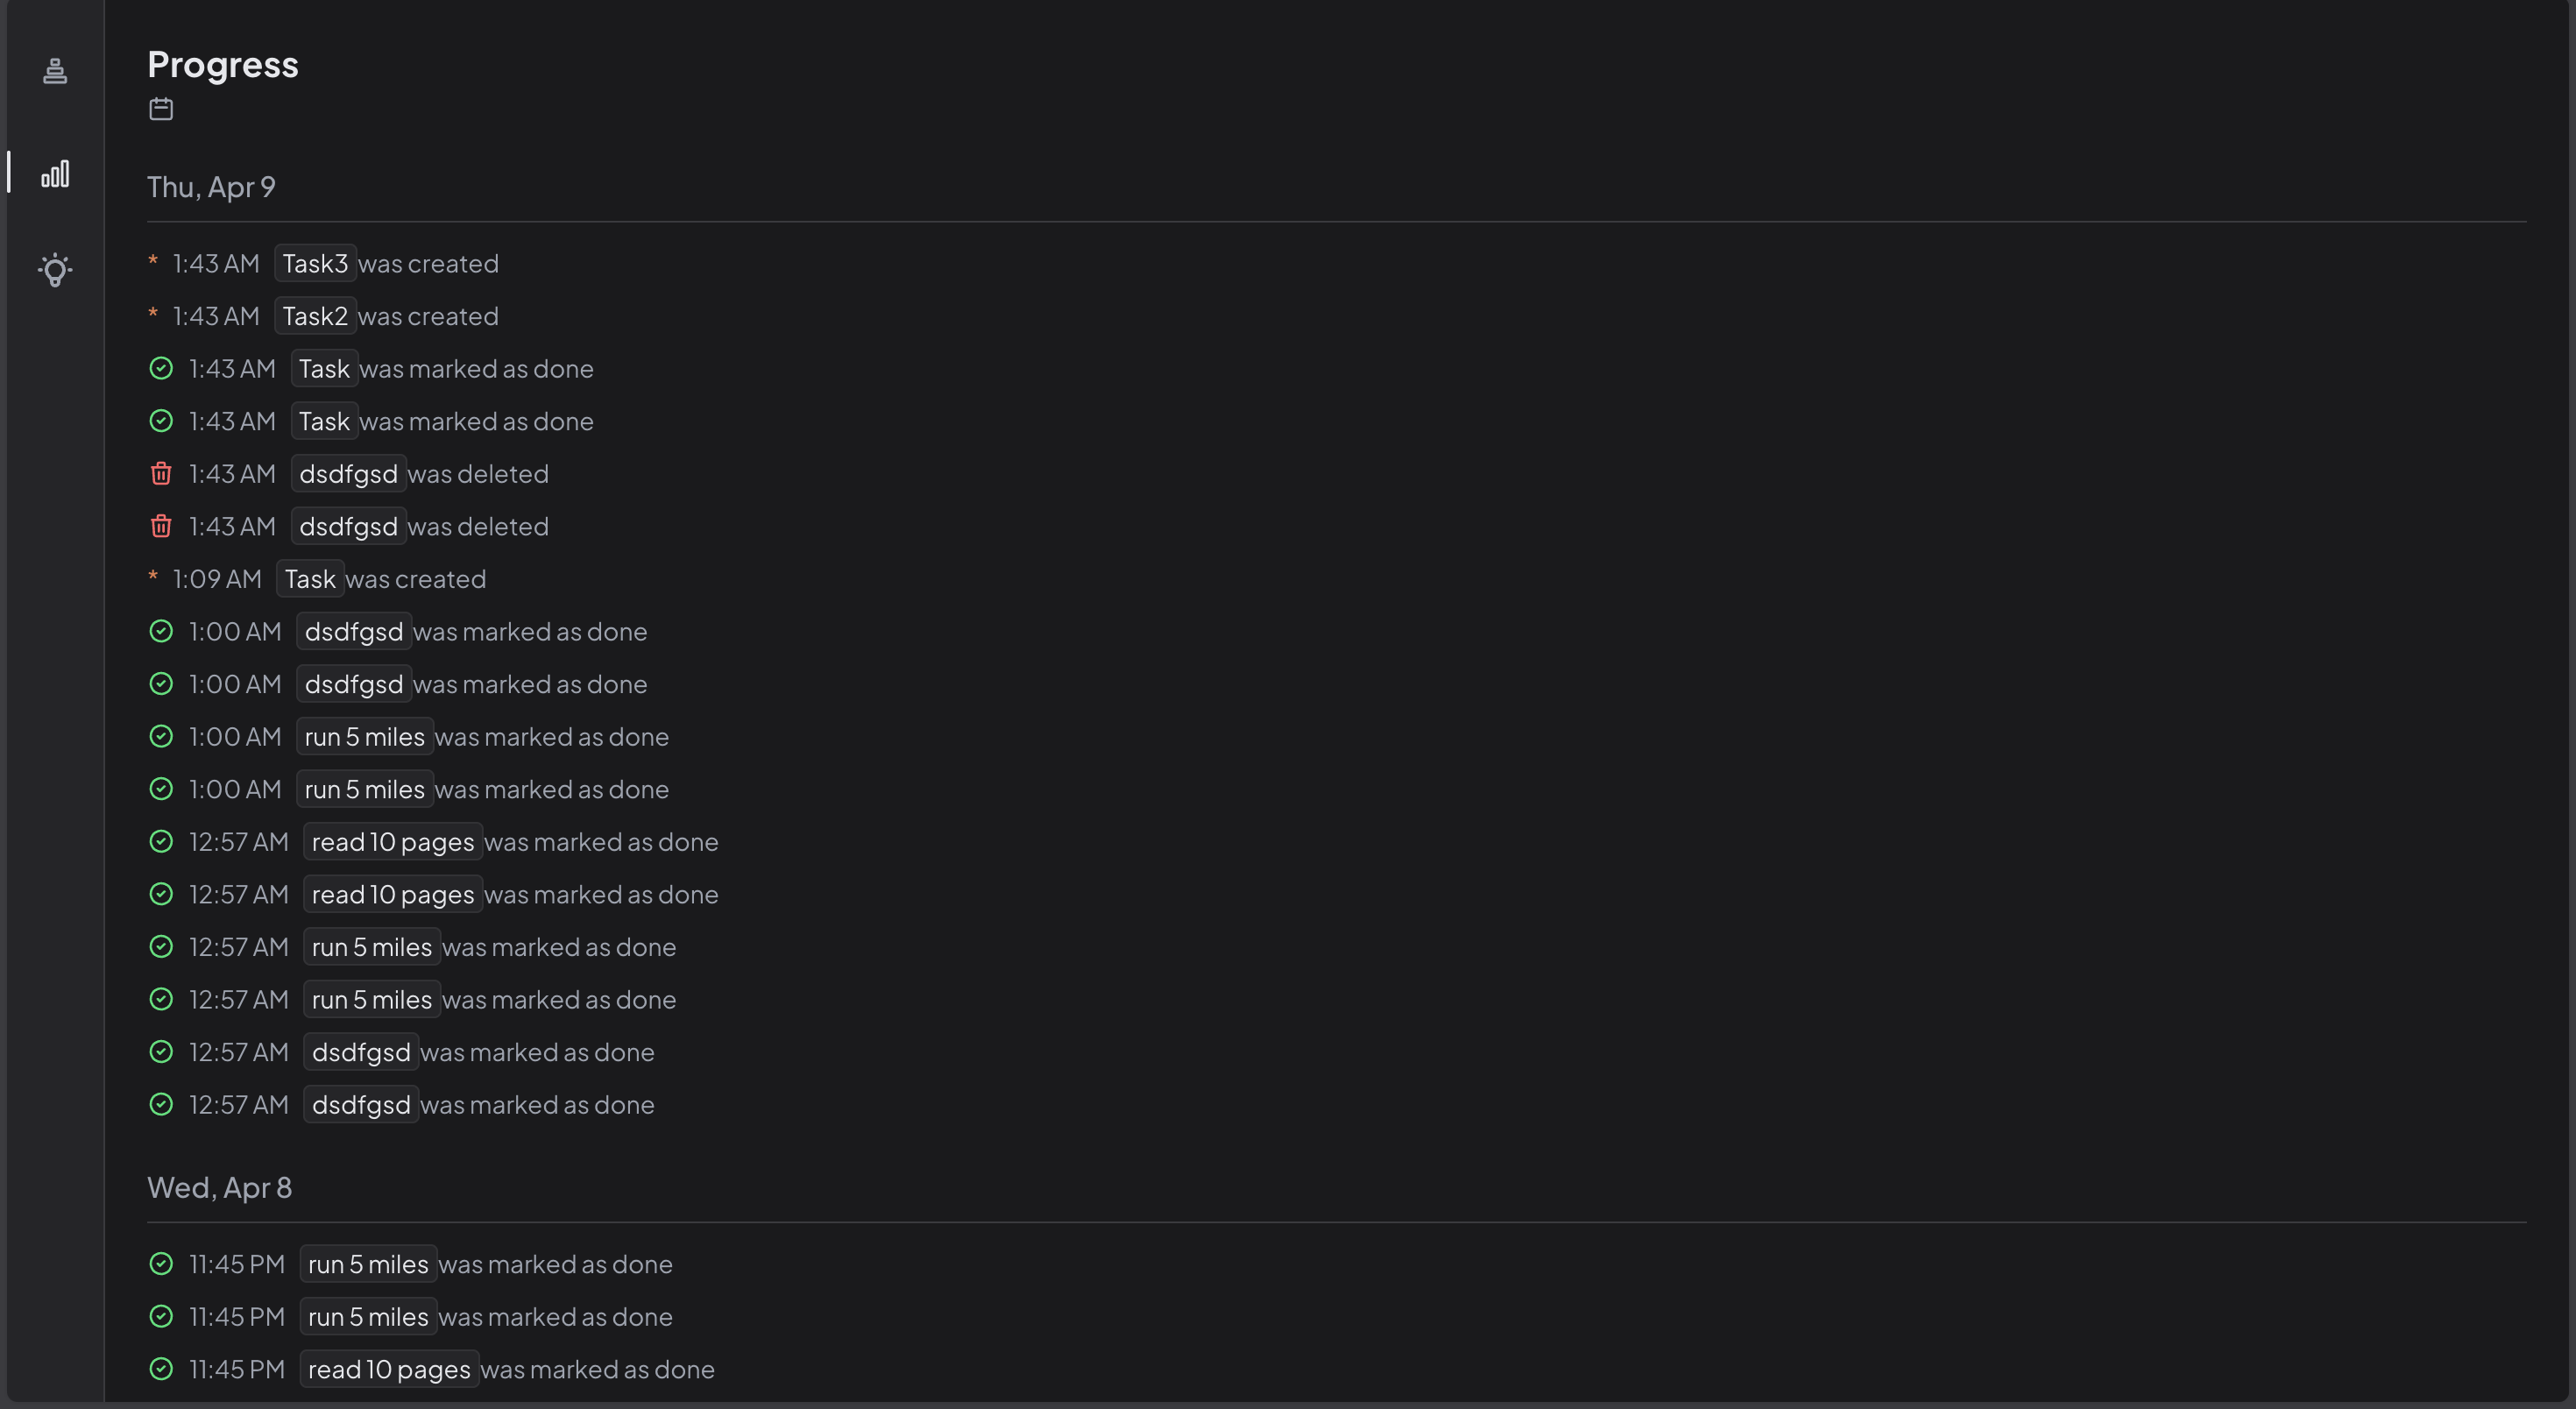
\includegraphics[width=0.8\linewidth]{ProgressPanel.png}
  \caption{Progress Panel}
  \label{fig:progress}
\end{figure}

\begin{figure}[h]
  \centering
  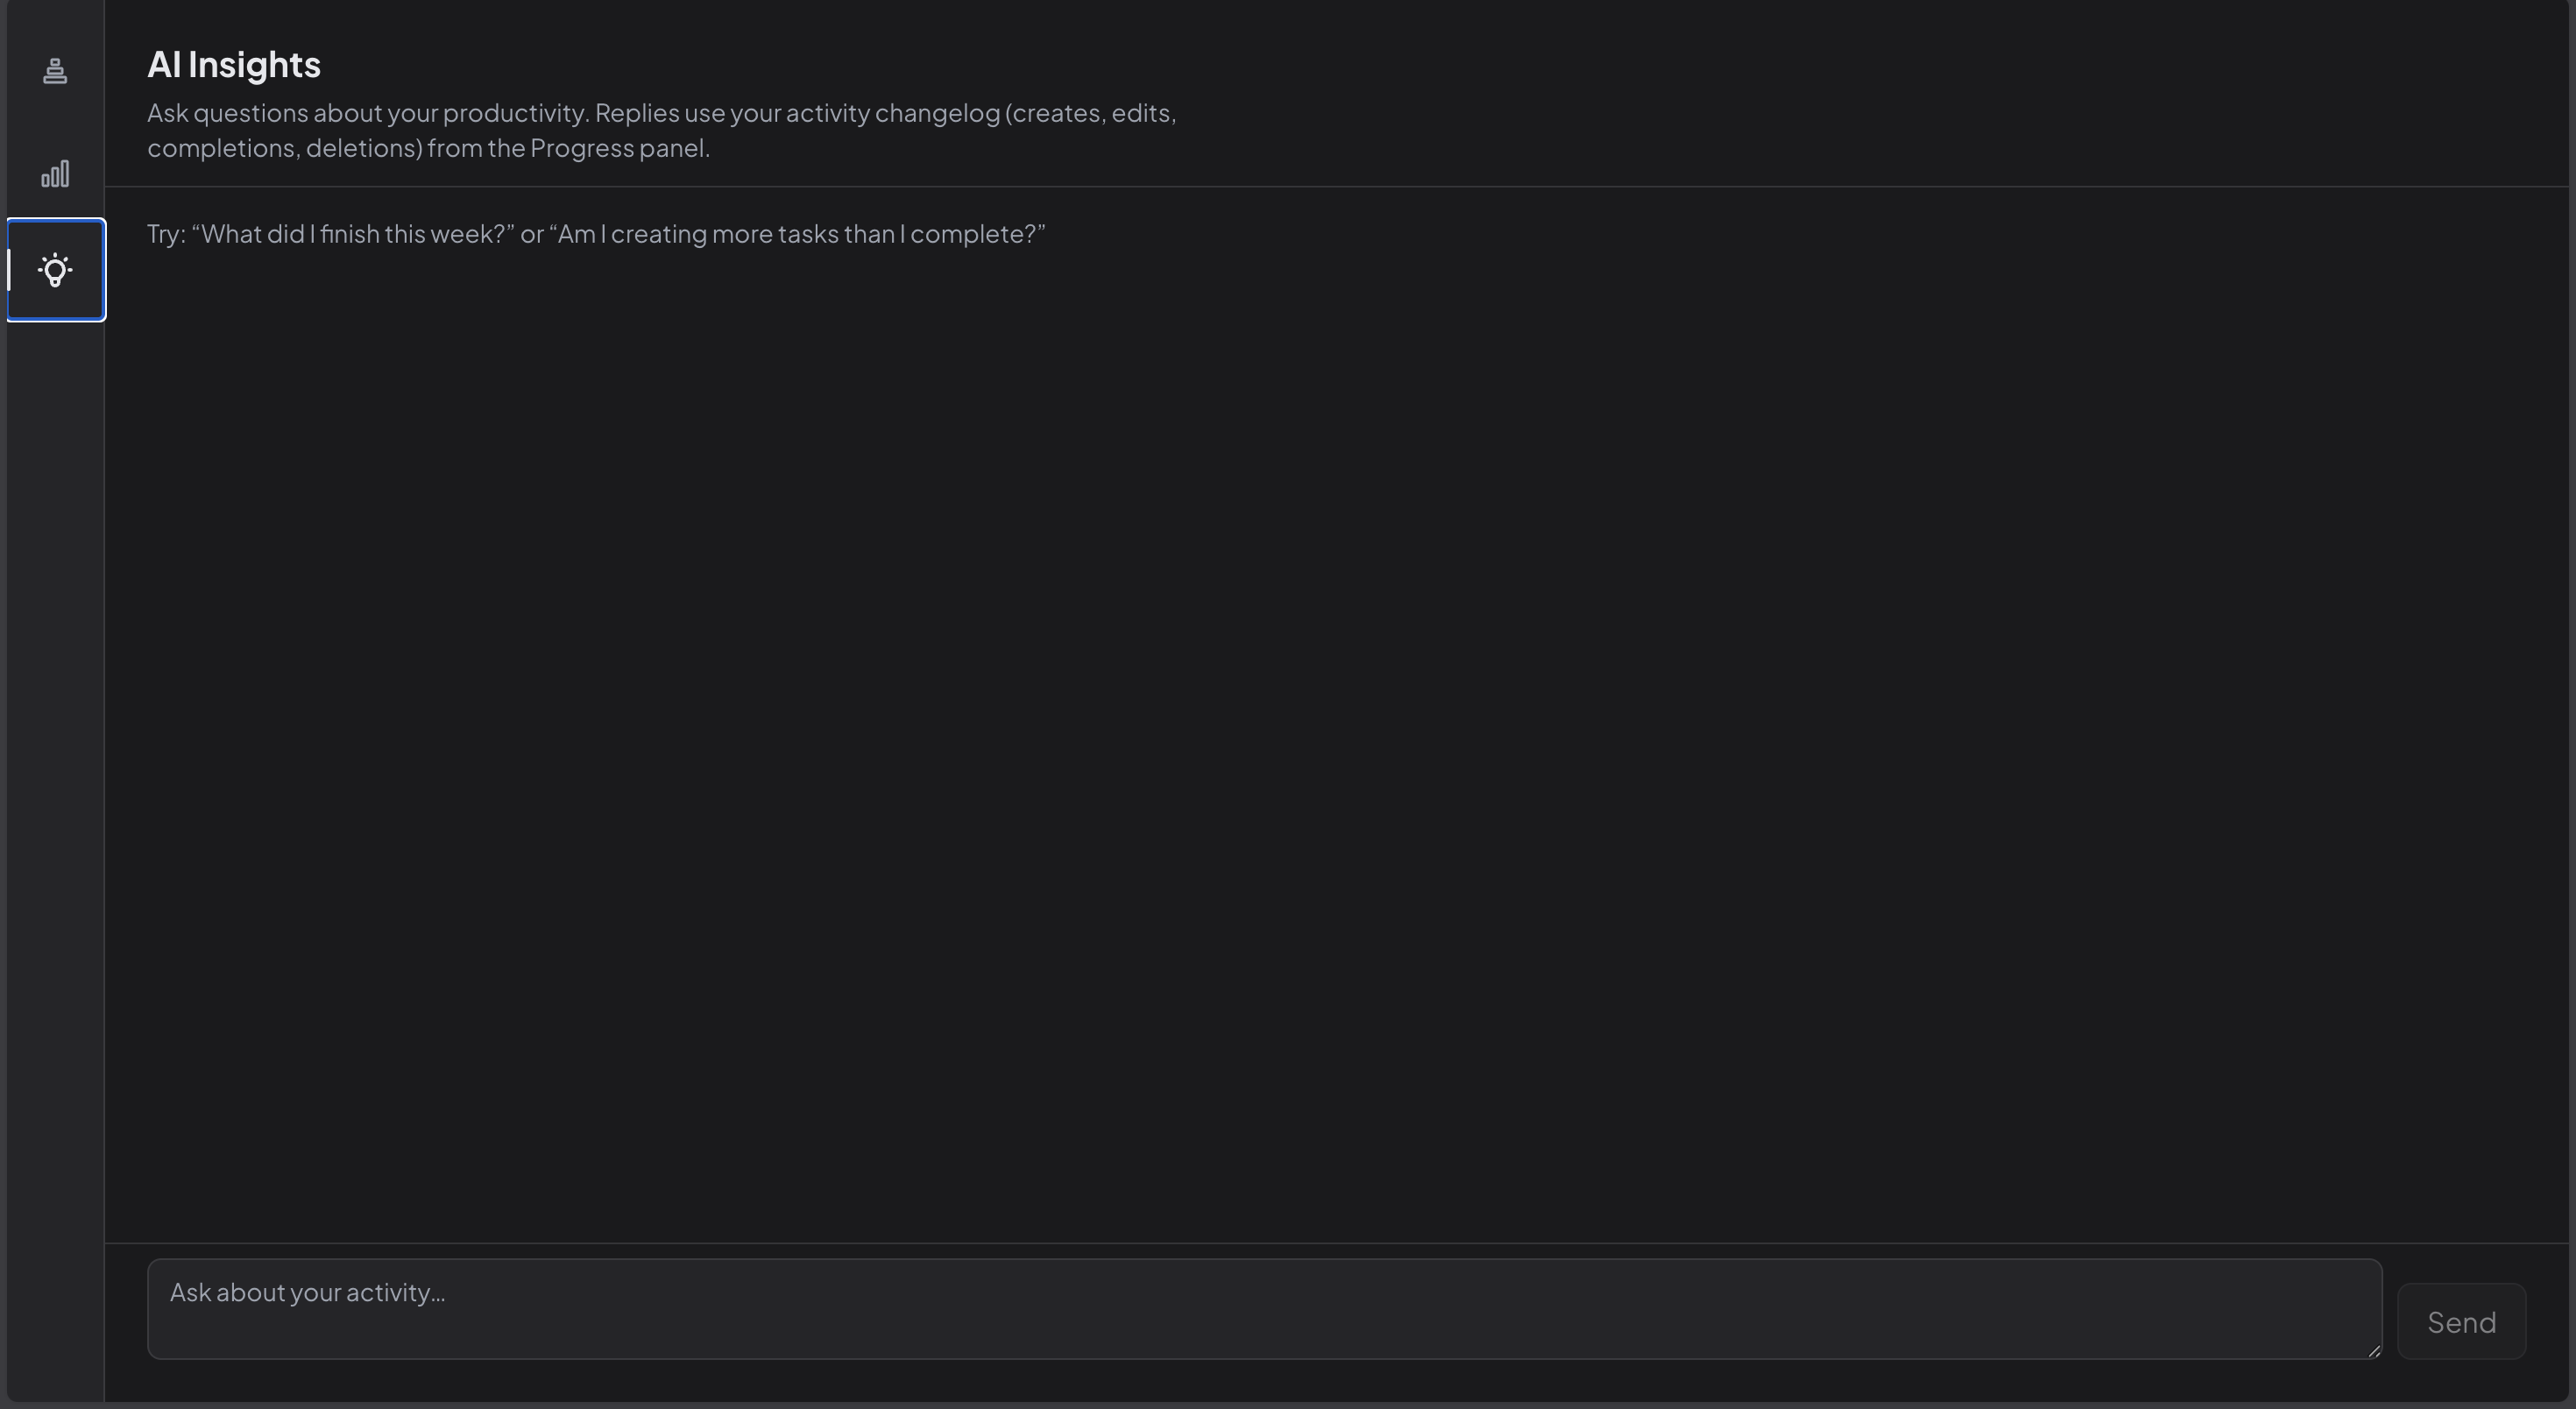
\includegraphics[width=0.8\linewidth]{AIReflection.png}
  \caption{AI Reflection}
  \label{fig:reflection}
\end{figure}

\begin{figure}[h]
  \centering
  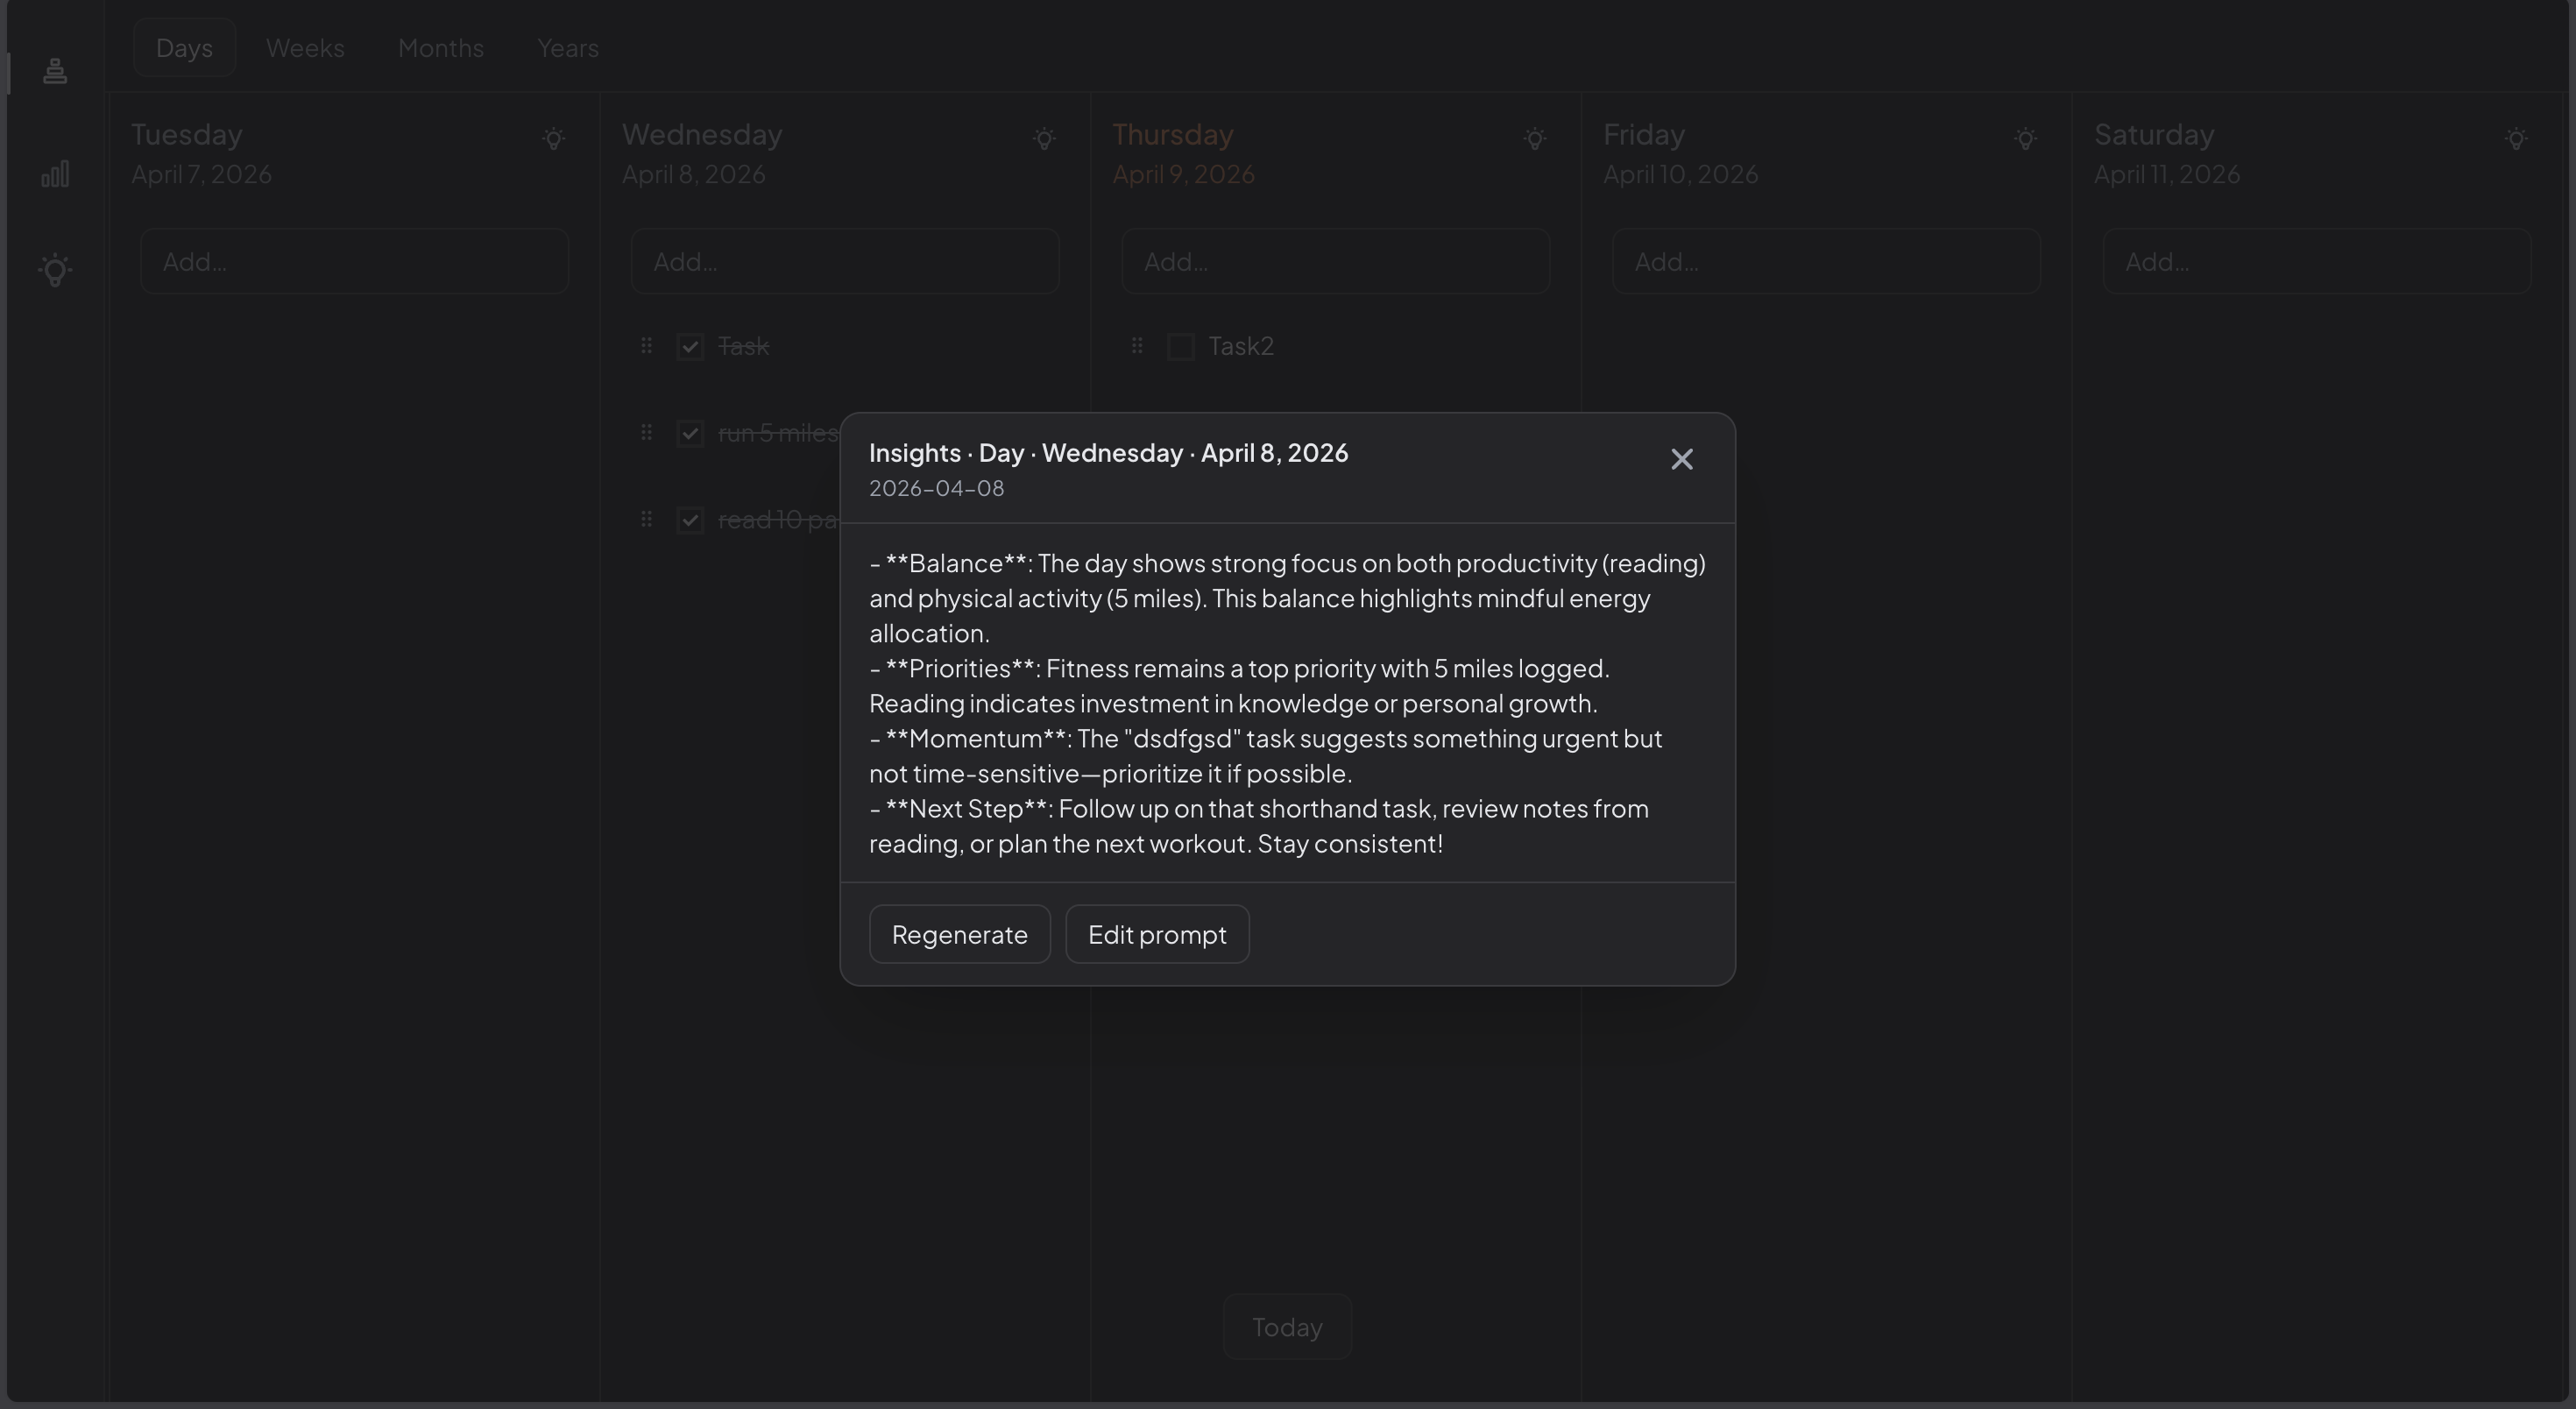
\includegraphics[width=0.8\linewidth]{insight-modal.png}
  \caption{AI-Insight Modal}
  \label{fig:insight}
\end{figure}



\bibliographystyle{acm}
\bibliography{bibliography.bib}

\end{document}
